% Vietnamese translation for OI Public Library
% Source-File: IOI中国国家候选队论文/2008/Day1/2.郑暾《平衡规划——浅析一类平衡思想的应用》/平衡规划.doc
\documentclass[11pt]{article}
\usepackage{tikz}
\usepackage{oipl-vn}

\newcommand{\Oh}{\mathcal{O}}

\tikzset{
  graphv/.style={circle,draw,fill=white,inner sep=1pt,minimum size=0.28cm},
  treev/.style={circle,fill=black,inner sep=1.35pt},
  matched/.style={line width=1.2pt},
  freeedge/.style={dashed},
  chain/.style={line width=1.25pt}
}

\title{Quy hoạch cân bằng\\{\large Bàn sơ về ứng dụng của một lớp tư tưởng cân bằng trong thi tin học}}
\author{Zheng Dun\\Trường Trung học số 8 Phúc Châu, Phúc Kiến}
\date{}

\begin{document}
\maketitle

\origtitle{Balanced Planning: an analysis of balance thinking in informatics competitions}
\sourcepath{IOI China candidate team papers / 2008 / Day 1 / Zheng Dun / balanced planning.doc}

\renewcommand{\abstractname}{Tóm tắt}
\begin{abstract}
Trọng tâm của việc giải bài bằng máy tính là thiết kế thuật toán, nhưng phạm
vi của thiết kế thuật toán rất rộng. Ta không thể kỳ vọng mình sẽ vận dụng
hoàn hảo mọi thuật toán; điều đáng quan tâm hơn thường là dùng hợp lý kiến
thức đã có, xây dựng một sự cân bằng giữa các thuật toán đã nắm, và giải được
càng nhiều bài càng tốt trong thời gian giới hạn. Bài viết này thử bàn về
một kiểu tư tưởng cân bằng trong cấu trúc thuật toán và trong hiện thực
chương trình.
\end{abstract}

\noindent\textbf{Từ khóa:} tư tưởng cân bằng, điểm cân bằng, hiệu quả thời
gian và bộ nhớ, độ phức tạp lập trình.

\section{Dẫn nhập}

``Cân bằng'' thường chỉ một trạng thái của vật thể hay hệ thống. Khi một vật
thể hay hệ thống đang ở trạng thái cân bằng, nếu không chịu tác động từ bên
ngoài thì tự nó sẽ không phát sinh thay đổi. Việc nhiều trạng thái đạt được
cân bằng thường là mục tiêu mà ta theo đuổi.

Tư tưởng cân bằng là một tư tưởng rất thú vị và có phạm vi ứng dụng rộng.
Trong thiết kế thuật toán, thiết kế cấu trúc dữ liệu, thậm chí trong lập
trình, ta đều có thể thấy bóng dáng của nó. Thi tin học là một cuộc chơi có
tính đối kháng; tìm điểm cân bằng trong cuộc chơi ấy, rồi dùng hợp lý tư
tưởng cân bằng để hỗ trợ thiết kế thuật toán và hiện thực chương trình,
thường có thể biến một cách làm tưởng như vụng về thành một lời giải hữu
dụng.

Trong thi tin học, tư tưởng cân bằng thường xuất hiện ở vài phương diện sau.
\begin{enumerate}
  \item \textbf{Bài toán trò chơi.} Nhiều bài toán trò chơi có thể chuyển
  thành việc tìm điểm cân bằng.
  \item \textbf{Xây dựng cấu trúc dữ liệu.} Mỗi cấu trúc dữ liệu hỗ trợ tốt
  một số thao tác nhất định. Chọn cấu trúc dữ liệu hợp lý thường có nghĩa là
  tăng nhẹ độ phức tạp của vài thao tác để giảm độ phức tạp của phần lớn thao
  tác còn lại, tức là dựng một sự cân bằng giữa hiệu quả của các thao tác.
  \item \textbf{Thời gian so với bộ nhớ.} Ta thường gặp những bài toán có
  thuật toán rất tốt về thời gian nhưng rất kém về bộ nhớ, hoặc ngược lại.
  Thiết kế thuật toán và tổ chức dữ liệu sao cho cân bằng được hai mặt này là
  điểm then chốt.
  \item \textbf{Thời gian, bộ nhớ so với các yếu tố khác.} Khi gặp bài khó,
  có lúc ta không thiết kế được thuật toán đẹp; cũng có lúc thuật toán hiệu
  quả đã có nhưng quá khó cài đặt trong phòng thi. Dùng quy hoạch cân bằng để
  xử lý những tình huống này thường đem lại hiệu quả bất ngờ. Đây cũng là
  trọng tâm của bài viết.
\end{enumerate}

Phần sau bàn về ba mẫu thường gặp: hiện thực không điển hình của thuật toán
kinh điển, thuật toán không hoàn hảo nhưng có hiệu quả tốt, và cấu trúc hóa
đơn giản cho bài toán phức tạp.

\section{Hiện thực không điển hình của thuật toán kinh điển}

Phần lớn thuật toán kinh điển đã quen thuộc với nhiều người, nhưng một thuật
toán kinh điển thường cũng có nhiều cách hiện thực khác nhau. Chẳng hạn, với
sắp xếp topo, nếu kích thước dữ liệu lớn ta thường dùng chương trình
\(\Oh(n)\); nếu kích thước nhỏ, một phiên bản ngắn dưới mười dòng theo cách
đơn giản hơn có thể làm mã nguồn sáng sủa hơn. Chỉ một khác biệt nhỏ trong
cách hiện thực cũng có thể dẫn đến khác biệt lớn về hiệu năng.

Hơn nữa, có những thuật toán dù là kinh điển nhưng có độ phức tạp tư duy và
độ phức tạp lập trình khá cao. Trong điều kiện phòng thi, một phương pháp
tương đối đơn giản và thực dụng thường là lựa chọn đáng cân nhắc.

\subsection{Ví dụ 1: Sắp xếp lịch cho bảo vệ, URAL 1099}

\textbf{Mô tả.} Cho quan hệ có thể làm việc chung giữa các bảo vệ. Cần ghép
các bảo vệ thành từng cặp để trực, và hỏi số bảo vệ tối đa có thể được sắp
lịch. Số bảo vệ không vượt quá \(222\).

\textbf{Phân tích ban đầu.} Bản chất của bài là tìm ghép cặp cực đại trên đồ
thị tổng quát. Thuật toán kinh điển là thuật toán blossom, với độ phức tạp
đa thức đủ tốt cho giới hạn này. Tuy nhiên blossom phức tạp cả về ý tưởng
lẫn lập trình, rất dễ cài sai hoặc suy biến, nên khó hoàn thành trong thời
gian thi. Vì vậy ta xét một thuật toán thay thế.

Khi giải ghép cặp cực đại trên đồ thị hai phía, thao tác chính là liên tục
tìm cây tăng luân phiên rồi điều chỉnh. Với đồ thị tổng quát, cách làm này
không luôn đúng. Trong sơ đồ dưới đây, các cạnh đậm là cạnh đã ghép, các cạnh
nét đứt là cạnh chưa ghép. Nếu cây tăng đang xét có dạng ở bên phải thì cách
mở rộng đơn giản không tìm thấy đường tăng, dù trên thực tế vẫn tồn tại một
đường tăng như cấu hình bên trái. Tìm đường tăng bằng tìm kiếm tổng quát là
quá tốn kém.

\begin{center}
\begin{tikzpicture}[x=1cm,y=1cm,every node/.style={font=\small}]
  \node[graphv,label=left:\(s\)] (s) at (0,0) {};
  \node[graphv] (a) at (0.9,0.6) {};
  \node[graphv] (b) at (1.8,0.0) {};
  \node[graphv] (c) at (2.7,0.6) {};
  \node[graphv] (d) at (3.6,0.0) {};
  \node[graphv,label=right:\(t\)] (t) at (4.5,0.6) {};
  \draw[freeedge] (s)--(a);
  \draw[matched] (a)--(b);
  \draw[freeedge] (b)--(c);
  \draw[matched] (c)--(d);
  \draw[freeedge] (d)--(t);
  \node at (2.25,-0.55) {hình 1: có đường tăng};

  \node[graphv,label=left:\(r\)] (r) at (6.0,0.25) {};
  \node[graphv] (u) at (7.0,0.95) {};
  \node[graphv] (v) at (7.0,-0.45) {};
  \node[graphv] (w) at (8.0,0.25) {};
  \node[graphv,label=right:\(z\)] (z) at (9.0,0.25) {};
  \draw[freeedge] (r)--(u);
  \draw[freeedge] (r)--(v);
  \draw[matched] (u)--(v);
  \draw[freeedge] (u)--(w);
  \draw[freeedge] (v)--(w);
  \draw[freeedge] (w)--(z);
  \node at (7.6,-0.95) {hình 2: cây luân phiên bị kẹt};
\end{tikzpicture}
\end{center}

Một quan sát quan trọng là: với cách điều chỉnh theo đường tăng, nếu một đỉnh
đã từng được ghép, thì sau các lần điều chỉnh nó vẫn có thể được ghép. Vì
vậy, với một đỉnh chưa ghép, việc có tìm được đường tăng bắt đầu từ nó hay
không là chìa khóa để cải thiện lời giải. Khả năng tìm được cây tăng lại phụ
thuộc mạnh vào thứ tự mở rộng trước đó; các dữ liệu làm hỏng cách tìm này
thường cũng dựa vào một thứ tự mở rộng đặc biệt. Điều đó gợi ý dùng thứ tự
mở rộng ngẫu nhiên để tránh các cấu hình đặc biệt như trong sơ đồ trên.

Chương trình của tác giả sinh hai hoán vị ngẫu nhiên: một cho thứ tự thăm
đỉnh lần đầu, một cho thứ tự mở rộng. Sau đó chương trình dùng trực tiếp
cách tìm cây luân phiên như đã nói, đồng thời chạy nhiều lần để tăng xác
suất gặp nghiệm tối ưu. Với giới hạn \(222\) đỉnh của URAL, phiên bản ban
đầu thường phải chạy \(20\) đến \(50\) lần mới tương đối chắc AC; con số này
khá lớn so với kích thước dữ liệu, cho thấy thuật toán còn nhiều yếu tố bất
định.

\subsubsection{Giới hạn số lần thất bại}

Nếu một đỉnh chưa được ghép trước đó, trong lượt tìm hiện tại nó rất có thể
vẫn sẽ chưa được ghép. Sai lệch cuối cùng thường đến từ việc một đỉnh vốn nên
được ghép lại bị bỏ qua vì một lần tìm cây tăng thất bại. Cách ban đầu giải
quyết bằng chạy lại toàn cục, tức là đôi khi phải làm lại tất cả chỉ vì một
đỉnh. Thay vào đó, ta có thể đổi thứ tự mở rộng và tìm lại cây luân phiên
ngay cho đỉnh vừa thất bại. Vì nhiều đồ thị không có ghép hoàn hảo, ta đặt
một ngưỡng số lần thất bại; chỉ khi vượt ngưỡng ấy mới bỏ đỉnh hiện tại.

Thí nghiệm trên hệ chấm URAL 1099, giới hạn thời gian \(0.5\) giây, cho kết
quả sau. Ký hiệu \(N-M\) nghĩa là chạy lặp \(N\) lần và đặt ngưỡng thất bại
là \(M\).

\[
\begin{array}{c|rrrrrrr}
\text{tham số} & 5\!-\!5 & 5\!-\!10 & 10\!-\!1 & 10\!-\!10 & 20\!-\!1 & 20\!-\!10 & 50\!-\!1 \\
\hline
\text{Accepted} & 90\% & 100\% & 0\% & 90\% & 60\% & 0\% & 100\% \\
\text{Wrong answer} & 10\% & 0\% & 100\% & 10\% & 40\% & 0\% & 0\% \\
\text{Time limit exceeded} & 0\% & 0\% & 0\% & 0\% & 0\% & 100\% & 0\% \\
\text{thời gian AC TB} & 0.0761 & 0.1471 & {-} & 0.2960 & 0.0385 & {-} & 0.0795
\end{array}
\]

Bảng cho thấy cách đặt ngưỡng thất bại làm tăng đáng kể xác suất ra nghiệm
tối ưu trong một lần chạy. Thuật toán ban đầu đến tham số \(20-1\) mới có tỉ
lệ AC quá một nửa, còn bản tối ưu với ngưỡng \(5\) đã đạt \(90\%\) khi chỉ
chạy \(5\) lần. Tất nhiên, do vẫn là thuật toán ngẫu nhiên và bộ dữ liệu
URAL khá mạnh, kết quả không đơn điệu tuyệt đối: chẳng hạn \(5-10\) đạt
\(100\%\) nhưng \(10-10\) chỉ đạt \(90\%\).

Đổi lại, phiên bản tối ưu có độ chính xác cao hơn nhưng tốn thời gian hơn.
Trong thí nghiệm, thời gian của \(5-5\) đã gần với \(50-1\); trường hợp
\(20-10\) đều quá thời gian cho thấy hệ số tăng không nhỏ. Về lý thuyết ta
chỉ nhân thêm một hằng số là ngưỡng thất bại, nhưng việc dùng nhiều hàm ngẫu
nhiên làm hằng số thực tế khá lớn.

\subsubsection{Mở rộng ý tưởng}

Thứ tự tìm kiếm ngẫu nhiên và giới hạn số lần thất bại không chỉ dùng cho
bài này. Nhìn bề ngoài, thứ tự ngẫu nhiên tránh các dữ liệu phụ thuộc vào
thứ tự. Bản chất của nó là gán thêm một số trọng số ngẫu nhiên để thay đổi
thuộc tính của trạng thái hiện tại, từ đó tránh sinh ra trường hợp đặc biệt.
Treap và quicksort ngẫu nhiên cũng dựa trên tinh thần này.

Giới hạn thất bại là một cách cải thiện độ chính xác của tìm kiếm ngẫu nhiên.
Thuật toán ngẫu nhiên vẫn có thể không đạt trạng thái mong muốn, ví dụ không
tìm ra đường tăng đang tồn tại, hoặc Treap không hoàn toàn cân bằng. Chạy lại
toàn cục làm tăng xác suất nghiệm tốt, còn giới hạn thất bại tập trung cải
thiện một vấn đề cục bộ để tăng xác suất đạt mục tiêu toàn cục. Kiểm tra số
nguyên tố lớn là một ứng dụng tương tự.

Với bài này, cả hai cách đều có thể qua được. Vì dữ liệu không lớn, nếu muốn
độ chính xác cao có thể tăng tham số; nếu muốn đảm bảo thời gian thì giảm
tham số. Ta đánh đổi độ chính xác để có một thuật toán tham lam ngẫu nhiên,
rồi lại đánh đổi thời gian để nâng xác suất đúng. Trong cả hai trường hợp,
độ phức tạp tư duy và lập trình đều giảm đáng kể.

\subsection{Ví dụ 2: Jackpot, PKU 2103}

\textbf{Mô tả.} Chọn một số nguyên theo mô hình giới hạn xác suất của đề bài.
Nếu số ấy chia hết cho ít nhất một trong các số \(p_1,p_2,\ldots,p_n\) thì
thắng. Với \(n\le 16\), cần tính xác suất thắng dưới dạng phân số tối giản.

\textbf{Phân tích ban đầu.} Đề bài đưa ra công thức giới hạn
\[
  P=\lim_{k\to\infty}\frac{S_k}{2k+1},
\]
trong đó \(S_k\) là số số nguyên từ \(-k\) đến \(k\) chia hết cho ít nhất một
trong các \(p_i\). Tính trực tiếp theo công thức này không tiện. Bài còn cần
số nguyên lớn, trong khi giới hạn thời gian khá chặt; nếu dùng số lớn thông
thường, hằng số dễ trở thành nút thắt.

Bài toán tương đương với việc xét một chu kỳ độ dài
\(\operatorname{lcm}(p_1,p_2,\ldots,p_n)\). Vì \(1\le p_i\le 10^9\), bội
chung nhỏ nhất có thể rất lớn, không thể quét trực tiếp. Nhưng chỉ có tối đa
\(16\) số, nên ta dùng nguyên lý bao hàm - loại trừ để đếm số vị trí thắng
trong một chu kỳ. Một mẹo là giữ trạng thái qua danh sách các số nguyên tố và
số mũ của chúng, rồi đến cuối mới khôi phục thành số nguyên lớn. Khi thuật
toán chính đã cố định, chất lượng hiện thực số lớn trở thành yếu tố quyết
định hiệu năng.

Phép toán số lớn thường dùng nhất ở đây là nhân số lớn với số nhỏ và cộng
trừ số lớn. Tối ưu quen thuộc là nén chữ số: trong phạm vi \texttt{longint}
thường nén \(4\) chữ số thập phân, còn với \texttt{int64} có thể nén \(8\)
chữ số. Nén làm giảm độ dài mảng, nhưng khi hiện thực lại phải dùng nhiều
phép \texttt{div} và \texttt{mod}, vốn có hằng số lớn. Ta có thể tránh chúng
bằng cách nén theo cơ số nhị phân.

Hai đoạn giả mã cho phép nhân số lớn với số nhỏ có cấu trúc gần như giống
nhau:

\noindent\textbf{Nén theo cơ số \(B=10^m\):}
\begin{verbatim}
for i = 1 .. a[0] + 1:
    p = a[i] * b + carry
    carry = p div B
    a[i] = p mod B
\end{verbatim}

\noindent\textbf{Nén theo cơ số \(B=2^t\):}
\begin{verbatim}
for i = 1 .. a[0] + 1:
    p = a[i] * b + carry
    carry = p shr t
    a[i] = p and (B - 1)
\end{verbatim}

Khi \(B=2^t\), phép chia và lấy dư được thay bằng dịch bit và phép
\texttt{and}. Độ dài mảng sau nén không kém nén thập phân, thậm chí có thể
tốt hơn, nên trong thực tế hiệu quả khá cao. Chương trình của tác giả dùng
cách này và qua toàn bộ dữ liệu trong một giây.

Cái giá phải trả là kết quả cuối cùng thường phải in ở hệ thập phân. Với cơ
số \(2^t\), không thể in trực tiếp từng khối như khi dùng cơ số \(10^m\); ta
cần thêm bước lấy dư theo \(10\) hoặc chuyển đổi hệ cơ số. Tuy vậy số lần in
thường rất ít, còn số lần tính toán số lớn trong bài lại nhiều, nên việc
tăng độ phức tạp ở đầu ra để giảm hằng số của phép toán chính là một cân
bằng có lợi.

Nhiều thuật toán kinh điển khác cũng có khó khăn tương tự: bản thân thuật
toán vốn dùng để đơn giản hóa bài toán, nhưng cách hiện thực lại trở thành
chướng ngại. Căn cứ vào nhu cầu thực tế, cải tạo thuật toán và chăm chút chi
tiết hiện thực để cân bằng độ phức tạp giữa các phần thường là vũ khí hữu
hiệu.

\section{Thuật toán không hoàn hảo nhưng có hiệu quả tốt}

Trong phòng thi, gặp bài không biết làm là chuyện rất thường gặp. Nhưng bỏ
qua hẳn một bài cũng đáng tiếc, vì một bài \(100\) điểm có thể ảnh hưởng
trực tiếp đến kết quả. Nếu đề có điểm từng phần, hoặc yêu cầu tìm nghiệm tối
ưu hay dựng phương án tối ưu, một thuật toán không hoàn hảo hoặc xấp xỉ đôi
khi đem lại kết quả tốt, dù không chắc đạt trọn điểm. Nếu có thể dùng quy
hoạch động hay tham lam để dựng một thuật toán ``gần đúng'' thì ta tiết kiệm
được nhiều thời gian suy nghĩ, tạo được cân bằng giữa số điểm thu được và
thời gian bỏ ra.

\subsection{Ví dụ 3: Truy bắt tên trộm, NOI 2007 Day 2}

\textbf{Mô tả.} Magic Land gồm \(N\) thành phố và \(N-1\) con đường, tạo
thành một cây. Tên trộm Frank có thể di chuyển trên đường với tốc độ tùy ý.
Ta không biết Frank đang ở thành phố nào hay trên con đường nào, nên phải
lập kế hoạch truy bắt. Mỗi đơn vị thời gian có thể làm một trong ba việc:
thả một thám tử xuống một thành phố, gọi một thám tử ở thành phố về tổng
hành dinh, hoặc cho một thám tử đi dọc một cạnh sang thành phố kề. Nếu thám
tử và Frank ở cùng thành phố hoặc gặp nhau trên cùng con đường thì bắt được
Frank. Cần dùng số thám tử ít nhất, với số bước không quá \(20000\).

Bài nhìn qua không quá phức tạp nhưng thực tế là bài khó nhất của kỳ thi đó.
Nó liên quan tới bài toán \emph{search number} trong lý thuyết đồ thị; với
đồ thị tổng quát bài toán là NP-khó, còn trên cây có thuật toán tuyến tính
cho giá trị và thuật toán \(\Oh(N\log N)\) cho phương án. Trong phòng thi,
không ai tìm ra lời giải chuẩn. Tuy nhiên cơ chế chấm có điểm từng phần và
chỉ cần một phương án hợp lệ cũng có điểm, nên một cấu trúc thay thế tốt vẫn
rất có giá trị.

\subsubsection{Ý tưởng cấu trúc}

Xét ví dụ nhỏ trong đề: thành phố \(2\) nối với \(1,3,4\). Một kế hoạch hợp
lệ là luôn để một thám tử ở thành phố \(2\), rồi lần lượt đưa một thám tử đi
quét các nhánh \(1\), \(3\), \(4\). Ví dụ này cho ta một ý tưởng quan trọng:
một đỉnh trên cây có thể chia cây thành nhiều phần độc lập. Nếu đặt một thám
tử thường trực ở đỉnh chia, Frank không thể đi từ phần này sang phần khác
mà không bị bắt. Do đó, khi tìm kiếm theo từng nhánh, thám tử giữ ở điểm
chia bảo vệ thành quả đã quét.

Ta có thể chọn một đỉnh để chia cây thành nhiều bài toán con. Nếu gọi
\(f(V)\) là số thám tử tốt, hoặc tối ưu, cho cây con có tập đỉnh \(V\), trực
giác chuyển trạng thái có dạng
\[
  f(V) \approx 1 + \max_i f(V_i),
\]
trong đó \(V_i\) là các thành phần sau khi bỏ đỉnh chia. Tuy nhiên trạng
thái con không dễ ghép: chọn điểm chia ra sao, ghép phương án của cây con
vào cây lớn thế nào, và làm sao tận dụng việc nhánh cuối cùng có thể dùng
luôn thám tử đang đứng ở điểm chia đều là các vấn đề khó.

Ta thay đổi mục tiêu: không cố đạt tối ưu tuyệt đối, mà dựng một phương án
khá tốt và dễ cài đặt. Chọn một điểm chia ban đầu làm gốc, dựng cây có gốc.
Với mỗi cây con, điểm chia được lấy luôn là gốc cây con. Khi xử lý các con,
ta để nhánh cần nhiều thám tử nhất làm nhánh cuối cùng, vì lúc đó một thám tử
đang giữ điểm chia có thể di chuyển xuống nhánh ấy mà không cần thêm người.
Chuyển trạng thái tham lam tương ứng là
\[
  D(x)=
  \begin{cases}
    1, & x \text{ là lá},\\
    \max\{2,\ \max_{y\in son(x)}D(y),\ 1+\operatorname{secondmax}_{y\in son(x)}D(y)\},
       & \text{ngược lại}.
  \end{cases}
\]
Ở đây \(D(x)\) là số thám tử khá tốt cho cây con gốc \(x\), còn
\(son(x)\) là tập các con của \(x\). Công thức thể hiện việc chỉ hai cây con
có nhu cầu lớn nhất mới ảnh hưởng trực tiếp đến số người cần đồng thời.

Khi dựng phương án, ta làm đúng theo chuyển trạng thái. Đặt hai thám tử ở
điểm chia, cử một thám tử đi xuống một con và đệ quy quét cây con đó; khi
quét đến lá thì thu hồi thám tử. Với mỗi điểm chia, cây con cần nhiều thám
tử nhất được xử lý sau cùng; khi đó không cần thả thêm người, mà cho thám tử
từ điểm chia đi xuống con tương ứng rồi tiếp tục đệ quy.

\subsubsection{Chất lượng lời giải}

Nhược điểm chính là ngoài điểm chia ban đầu được liệt kê, các cây con đều
lấy gốc cây con làm điểm chia. Điều này làm phương án dễ dựng nhưng có thể
không tối ưu. Sơ đồ phản ví dụ dưới đây biểu diễn một cây mà thuật toán tham
lam cần \(4\) thám tử, trong khi phương án tối ưu chỉ cần \(3\): giữ thám tử
ở \texttt{root}, phối hợp hai thám tử khác đi vào các nhánh sâu, thu hồi và
tái sử dụng họ theo thứ tự khéo léo. Vì thuật toán luôn chia cây con tại gốc
của nó nên không tìm được cấu trúc phối hợp ấy.

\begin{center}
\begin{tikzpicture}[x=0.85cm,y=0.8cm,every node/.style={font=\small}]
  \node[treev,label=above:{\texttt{root}}] (r) at (0,4) {};
  \foreach \x/\n in {-2/a,0/b,2/c} {
    \node[treev] (\n1) at (\x,3) {};
    \node[treev] (\n2) at (\x,2) {};
    \node[treev] (\n3) at (\x,1) {};
    \draw (r)--(\n1)--(\n2)--(\n3);
  }
  \node[treev] (a4) at (-2.6,0) {};
  \node[treev] (a5) at (-1.4,0) {};
  \draw (a3)--(a4) (a3)--(a5);
  \node[treev] (b4) at (-0.6,0) {};
  \node[treev] (b5) at (0.6,0) {};
  \draw (b3)--(b4) (b3)--(b5);
  \node[treev] (c4) at (1.4,0) {};
  \node[treev] (c5) at (2.6,0) {};
  \draw (c3)--(c4) (c3)--(c5);
  \node[align=center] at (0,-0.75)
    {chia tại gốc cây con dễ cần \(4\); phối hợp thứ tự quét có thể dùng \(3\)};
\end{tikzpicture}
\end{center}

Dù vậy thuật toán vẫn có ý nghĩa. Chất lượng nghiệm tại một đỉnh chỉ chịu
ảnh hưởng của hai cây con có nhu cầu lớn nhất; các cây con còn lại dù hơi
kém cũng không làm tăng đáp án cuối. Nói cách khác, lời giải có một khoảng
đàn hồi nhất định. Dữ liệu khắc chế cục bộ cũng khó dựng: một phản ví dụ đầy
đủ cần khoảng ba mươi đỉnh mới đủ hình dạng. Khi kích thước dữ liệu
tăng, dữ liệu ngẫu nhiên dù chứa vài cấu trúc xấu cũng khó ảnh hưởng đến
kết quả cuối. Việc liệt kê gốc ban đầu làm độ phức tạp tăng lên
\(\Oh(N^2)\), nhưng thời gian vẫn rộng rãi và chất lượng nghiệm tăng rõ.

Tác giả thử \(1000\) bộ dữ liệu ngẫu nhiên: khoảng \(85\%\) kết quả cần
\(5\) thám tử, phần còn lại cần \(6\) thám tử, rất hiếm khi chỉ cần \(4\).
Đối chiếu luật chấm, cách này ít nhất thường đạt \(60\%\) điểm; trong kỳ
thi, chương trình đạt \(96\) điểm, chỉ có một test nhiều hơn đáp án chuẩn
\(1\) thám tử.

Với một bài ở mức độ luận văn như vậy, \(96\) điểm trong phòng thi là kết quả
rất tốt. Cấu trúc này có độ phức tạp tư duy thấp, cài đặt nhẹ, thời gian vừa
phải và chất lượng nghiệm cao. Ta đánh đổi một phần chất lượng nghiệm để
giảm mạnh độ khó tư duy và hiện thực, rồi tối ưu hóa hợp lý trên nền phương
án đơn giản để thường đạt nghiệm tối ưu.

Trong lớp bài toán này, nếu vấn đề gốc quá khó, cố chấp theo đuổi AC trọn
vẹn có thể không hiệu quả. Một thuật toán xấp xỉ tốt tạo ra sự cân bằng giữa
điểm số và thời gian tiêu hao, nên cũng là một chiến lược thi đấu đáng giá.

\section{Cấu trúc hóa đơn giản cho bài toán phức tạp}

Không phải bài nào cũng có thuật toán xấp xỉ hữu hiệu như trên. Trong các
cuộc thi kiểu ACM, hoặc khi đề yêu cầu duy trì một chuỗi thao tác chính xác,
xấp xỉ thường không dùng được. Khi đó, nếu chưa tìm được thuật toán thật đẹp
về thời gian và bộ nhớ, ta cần bình tĩnh phân tích đặc điểm đề. Một phương
pháp thường dùng là chấp nhận hy sinh một phần hiệu quả thời gian hoặc bộ
nhớ trong giới hạn cho phép để giảm độ phức tạp tư duy và lập trình.

Những bài như vậy thường có một đặc điểm: nếu điều kiện đề mạnh hơn một chút
và giới hạn các trường hợp về một dạng đặc biệt, ta có thuật toán tốt; nhưng
khi mở rộng lên dạng tổng quát thì thuật toán ấy không dùng trực tiếp được.
Khai thác thông tin từ trường hợp đặc biệt để đơn giản hóa mô hình, tức là
dựng cân bằng giữa đặc biệt và tổng quát, thường là chìa khóa.

\subsection{Ví dụ 4: Duy trì dãy số}

\textbf{Mô tả.} Cho dãy số nguyên độ dài \(n\le 100000\), cần duy trì hai
thao tác:
\begin{enumerate}
  \item cộng một số nguyên vào mọi phần tử từ vị trí \(i\) đến \(j\);
  \item hỏi trong đoạn từ \(i\) đến \(j\) có bao nhiêu số nhỏ hơn \(c\).
\end{enumerate}
Số thao tác tối đa là \(10000\).

\textbf{Phân tích.} Bài yêu cầu cấu trúc dữ liệu cho thao tác đoạn vừa có so
sánh, truy vấn, vừa có cập nhật cộng. Phản xạ đầu tiên thường là dùng cây
lồng cây. Nhưng cập nhật biến đổi cả đoạn làm việc hợp nhất các cấu trúc con
không còn lý tưởng; hơn nữa cây lồng cây có mã nguồn lớn, khó gỡ lỗi, rủi ro
cao trong phòng thi. Vì số thao tác chỉ \(10000\) và thời gian \(5\) giây
không quá chặt, ta có thể chọn một thuật toán đơn giản hơn.

Khối liên kết là một cấu trúc quen thuộc cho thao tác đoạn, nhưng nếu viết
đầy đủ thì mã vẫn dài. Ý tưởng chia khối có thể được dùng theo dạng nhẹ hơn:
\term{mảng chia khối}. Ta chia trực tiếp mảng gốc thành khoảng
\(\sqrt n\) khối, mỗi khối dài khoảng \(\sqrt n\). Mỗi khối có thêm trường
ghi nhận phần cộng dồn hoặc thông tin thống kê. Cấu trúc này rất dễ hiện
thực bằng chính mảng gốc; nó thích hợp với các thao tác cộng đoạn và hỏi
thống kê đoạn, nhưng không hỗ trợ chèn xóa vì thứ tự phần tử phải cố định.
Bài này đúng với điều kiện đó.

Gọi \(A\) là mảng gốc và \(B\) là bản sao dùng cho từng khối theo thứ tự đã
sắp. Tiền xử lý: chia \(B\) thành \(\sqrt n\) khối, mỗi khối dài
\(\sqrt n\); sắp xếp từng khối tăng dần và đặt nhãn cộng dồn của khối bằng
\(0\).

Với thao tác cộng đoạn, ta xác định các khối nằm hoàn toàn trong đoạn. Những
khối này chỉ cần tăng nhãn cộng dồn. Hai khối biên, nếu có, được cập nhật
trực tiếp từng phần tử rồi sắp xếp lại khối. Mỗi thao tác nhiều nhất xử lý
\(\Oh(\sqrt n)\) khối nguyên và sửa \(\Oh(\sqrt n)\) phần tử biên; chi phí
sắp xếp lại hai khối là \(\Oh(\sqrt n\log n)\).

Với thao tác hỏi, các khối nằm hoàn toàn trong đoạn đang được giữ theo thứ
tự nên có thể dùng tìm kiếm nhị phân để đếm số phần tử nhỏ hơn
\(c-\text{tag}\). Hai khối biên được quét trực tiếp. Vì vậy một truy vấn
tốn \(\Oh(\sqrt n\log n)\) thời gian.

Tổng cộng với \(m\) thao tác, độ phức tạp xấp xỉ
\[
  \Oh(m\sqrt n\log n),
\]
ở mức vài chục triệu phép tính cho giới hạn đề, đủ để qua dữ liệu.

Bài này có thể có lời giải cây lồng cây với độ phức tạp tiệm cận đẹp hơn,
nhưng độ khó tư duy và hiện thực cao hơn nhiều. Nhờ giới hạn thao tác và
việc thứ tự dãy không thay đổi, mảng chia khối cân bằng được thời gian chạy
với độ phức tạp lập trình, đồng thời hằng số nhỏ.

\subsection{Ví dụ 5: Duy trì cây, PKU 3237}

\textbf{Mô tả.} Cho một cây \(N\) đỉnh, các đỉnh đánh số \(1\) đến \(N\),
các cạnh đánh số theo thứ tự nhập và có trọng số. Cần duy trì:
\begin{enumerate}
  \item \texttt{CHANGE i v}: đổi trọng số cạnh \(i\) thành \(v\);
  \item \texttt{NEGATE a b}: đổi dấu mọi cạnh trên đường đi từ \(a\) đến
  \(b\);
  \item \texttt{QUERY a b}: hỏi trọng số lớn nhất trên đường đi từ \(a\) đến
  \(b\).
\end{enumerate}
Số bộ dữ liệu không quá \(20\), số đỉnh không quá \(10000\).

\textbf{Phân tích ban đầu.} Đây là bài duy trì thao tác trên đường đi của
cây. Dynamic tree có vẻ rất phù hợp với độ phức tạp logarit, nhưng nó hơi
quá mạnh vì cây trong bài không đổi hình dạng. Hiện thực dynamic tree cũng
phức tạp và hằng số lớn. Vì vậy ta tìm một thuật toán thay thế.

Trước hết xét trường hợp đặc biệt: cây suy biến thành một đường thẳng. Khi
đó bài là bài segment tree quen thuộc. Mục tiêu là đưa bài toán trên cây về
các đoạn trên đường thẳng. Cố gắng lấy thứ tự DFS của cả cây làm một dãy
không thành công; nhưng ý tưởng chuyển cây thành các dây vẫn hữu ích. Nếu
không chuyển được thành một dây, ta tách cây thành nhiều dây.

Chọn tùy ý một gốc và đưa trọng số mỗi cạnh xuống đỉnh con của cạnh ấy. Với
một đỉnh \(x\), giả sử các con của nó đã thuộc các dây đi từ dưới lên và kết
thúc tại con tương ứng; ta nối \(x\) vào dây dài nhất trong các dây đó. Như
vậy mọi đỉnh thuộc đúng một dây tách, một số dây có thể chỉ có một đỉnh. Việc
đưa trọng số cạnh xuống đỉnh con giúp các cạnh bị cắt giữa hai dây không cần
xử lý riêng như cạnh độc lập.

Sơ đồ dưới đây minh họa một cây được tách thành năm dây; các cạnh đậm là cạnh
trong dây. Với mỗi dây, ta dựng một segment tree. Vì có thao tác đổi dấu, mỗi
nút segment tree cần giữ cả giá trị lớn nhất và nhỏ nhất. Quan hệ giữa các
dây có thể lưu bằng cấu trúc hợp nhất hoặc mảng đại diện.

\begin{center}
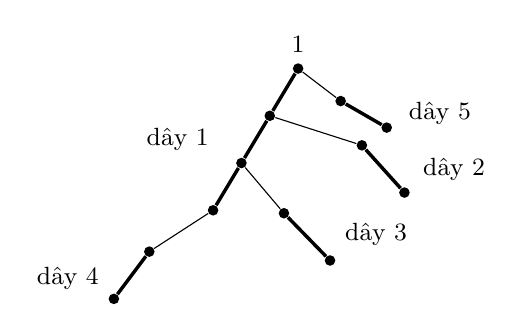
\begin{tikzpicture}[x=0.9cm,y=0.75cm,every node/.style={font=\small}]
  \node[treev,label=above:{1}] (r) at (0,4) {};
  \node[treev] (a) at (-0.4,3.2) {};
  \node[treev] (b) at (-0.8,2.4) {};
  \node[treev] (c) at (-1.2,1.6) {};
  \draw[chain] (r)--(a)--(b)--(c);
  \node at (-1.7,2.8) {dây 1};

  \node[treev] (d) at (0.9,2.7) {};
  \node[treev] (e) at (1.5,1.9) {};
  \draw (a)--(d);
  \draw[chain] (d)--(e);
  \node at (2.2,2.3) {dây 2};

  \node[treev] (f) at (-0.2,1.55) {};
  \node[treev] (g) at (0.45,0.75) {};
  \draw (b)--(f);
  \draw[chain] (f)--(g);
  \node at (1.1,1.2) {dây 3};

  \node[treev] (h) at (-2.1,0.9) {};
  \node[treev] (i) at (-2.6,0.1) {};
  \draw (c)--(h);
  \draw[chain] (h)--(i);
  \node at (-3.25,0.45) {dây 4};

  \node[treev] (j) at (0.6,3.45) {};
  \node[treev] (k) at (1.25,3.0) {};
  \draw (r)--(j);
  \draw[chain] (j)--(k);
  \node at (2.0,3.25) {dây 5};
\end{tikzpicture}
\end{center}

Ba thao tác được xử lý như sau.
\begin{enumerate}
  \item \texttt{CHANGE}: sửa giá trị tại đỉnh con tương ứng với cạnh đó, rồi
  cập nhật segment tree của dây chứa đỉnh ấy. Chi phí \(\Oh(\log m)\), với
  \(m\) là độ dài dây.
  \item \texttt{NEGATE}: tìm LCA của \(A\) và \(B\), rồi xử lý hai đường
  \(A\) đến LCA và \(B\) đến LCA. Mỗi lần đi qua một dây, thực hiện đổi dấu
  trên đoạn tương ứng của segment tree.
  \item \texttt{QUERY}: cũng tách thành hai đường qua LCA, lần lượt hỏi các
  đoạn trên các dây và lấy giá trị lớn nhất.
\end{enumerate}

Các thao tác tìm LCA, xác định đường và nhảy giữa các dây có thể làm trong
thời gian hằng số sau tiền xử lý phù hợp. Nút thắt là số dây mà một đường có
thể đi qua.

\subsubsection{Ước lượng số dây}

\textbf{Bổ đề.} Với cách tách dây tham lam ở trên, trên đường từ một đỉnh
\(x\) lên một tổ tiên \(\text{root}\), số dây tách xuất hiện không quá
\(\Oh(\sqrt n)\).

\textbf{Chứng minh.} Gọi \(S\) là tập các cạnh trên đường từ \(x\) đến
\(\text{root}\), và giả sử các cạnh trong \(S\) thuộc \(k\) dây. Xét các
đỉnh cao nhất nơi đường đi chuyển từ dây này sang dây khác. Vì tại mỗi điểm
chuyển, thuật toán đã chọn dây con dài nhất để nối lên cha, nên dây không
được chọn ở lần chuyển thứ \(i\) phải chứa ít nhất \(i\) đỉnh nằm ngoài
đường đang xét. Do đó cây con gốc \(\text{root}\) phải chứa ít nhất
\[
  1+2+\cdots+(k-1)=\frac{k(k-1)}{2}
\]
đỉnh ngoài phần chính, suy ra \(k=\Oh(\sqrt n)\). Bổ đề được chứng minh.

Từ bổ đề, thao tác \texttt{NEGATE} và \texttt{QUERY} đi qua nhiều nhất
\(\Oh(\sqrt n)\) dây, mỗi dây tốn \(\Oh(\log n)\) cho segment tree. Vì vậy
độ phức tạp xấu nhất của hai thao tác này là
\[
  \Oh(\sqrt n\log n).
\]
Với một bộ dữ liệu, chặn trên tổng thể nhìn có vẻ hơi căng, nhưng đây là
chặn rất rộng. Trong thực tế số dây đi qua thường nhỏ, hằng số của chương
trình thấp; chương trình của tác giả qua toàn bộ dữ liệu PKU trong \(951\)
ms. Tác giả cũng dùng phương pháp này để AC đầu tiên bài tương tự URAL 1553
trong một cuộc thi.

Ở đây ta bỏ dynamic tree với độ phức tạp logarit rất đẹp, thay bằng cách
tách cây thành dây rồi dùng segment tree. Bằng cách xét trường hợp đặc biệt
là một dây và mở rộng có kiểm soát lên cây, ta xây được sự cân bằng giữa
trường hợp đặc biệt và bài toán tổng quát. Dù chặn xấu nhất lớn hơn, hiệu
quả thực tế tốt và hiện thực đơn giản hơn nhiều.

\section{Tổng kết}

Có một ví dụ kinh điển về chiếc thùng gỗ: sức chứa của thùng không phụ thuộc
vào tấm gỗ dài nhất mà phụ thuộc vào tấm gỗ ngắn nhất. Nếu xem thời gian,
bộ nhớ và các yếu tố khác là những tấm gỗ của chiếc thùng ``giải bài'', thì
tấm gỗ ta thường bỏ quên chính là độ phức tạp tư duy và hiện thực. Muốn tăng
sức chứa, có thể cắt bớt tấm dài để bù cho tấm ngắn; khi các tấm gỗ gần bằng
nhau, sức chứa đạt mức tốt hơn. Tư tưởng cân bằng chính là kiểu lấy dài bù
ngắn đó.

Những bài phù hợp với tư tưởng cân bằng thường có một nút thắt chính. Bài
viết đã giới thiệu một lớp cách dùng tư tưởng cân bằng cho các nút thắt ấy,
đặc biệt là mô hình chấp nhận trả giá ở một mặt khác để giảm độ phức tạp tư
duy và lập trình. Bằng cách cân bằng nhiều loại độ phức tạp, ta có thể giải
được nhiều bài hơn trong thời gian hữu hạn. Trên sân thi, không nhất thiết
phải theo đuổi độ phức tạp thời gian và bộ nhớ hoàn mỹ nhất; điểm cao mới là
lẽ cứng, AC mới là lẽ cứng.

Nhìn từ bên ngoài, quy hoạch cân bằng có vẻ giống một tư tưởng ``kiếm điểm''.
Tác giả cho rằng giải bài tin học không chỉ là đơn thuần theo đuổi độ phức
tạp thời gian hoàn hảo. Trong thời gian hữu hạn, ta phải xét tổng hợp nhiều
yếu tố; đó cũng là sức hấp dẫn của thi tin học. Dùng hợp lý kiến thức đã học,
kết hợp chúng hiệu quả, quyết định hợp lý mô hình toán học và cách phân phối
công sức giữa thiết kế với hiện thực mới giúp giải bài hiệu quả. Dĩ nhiên,
điều này vẫn đòi hỏi nền tảng vững chắc để có nhiều lựa chọn hơn trong phòng
thi. Tư tưởng này cũng cần được rèn luyện qua thực hành; như câu cổ văn mà
tác giả dẫn: điều học được trên giấy vẫn còn nông, muốn hiểu sâu thì phải tự
thân làm.

\section*{Lời cảm ơn}

Tác giả cảm ơn Chen Danqi đã cung cấp một phần tài liệu và góp ý cho việc
hiện thực, chỉnh sửa bài viết; cảm ơn Dong Huaxing, Liu Yi đã góp ý chỉnh
sửa; cảm ơn huấn luyện viên Liu Rujia và các thầy Chen Guang, Hu Shanli đã
đưa ra góp ý cho việc hiện thực và chỉnh sửa.

\section*{Tài liệu tham khảo}

\begin{enumerate}
  \item Liu Rujia, Huang Liang, \emph{Nghệ thuật thuật toán và thi tin học}.
  \item Zhou Gelin, báo cáo lời giải \emph{Query on a tree} (SPOJ 375).
  \item Xu Zhilei, phân tích bài \emph{Catch}.
\end{enumerate}

\section*{Ghi chú về phụ lục nguồn}

Tài liệu gốc kèm toàn văn đề của URAL 1099, PKU 2103, NOI 2007
\emph{Catch} và PKU 3237. Các phụ lục dài này không được dịch nguyên văn ở
đây; nội dung cần thiết cho mạch phân tích đã được nêu gọn trong từng ví dụ.
Các hình minh họa cấu hình đồ thị hoặc cây đã được dựng lại bằng sơ đồ
TikZ gọn trong bản dịch.

\end{document}
